%
% summary landscape plots
%
      \begin{figure*}[t]
        \centering
        \begin{subfigure}[b]{0.45\textwidth}
            \centering
            \caption[]%
            {{\small Netpipe 64 KB message}}  
            \vspace*{-0.3cm}
            %\hspace*{0.35cm}  
            \label{fig:netpipe64Kov}
            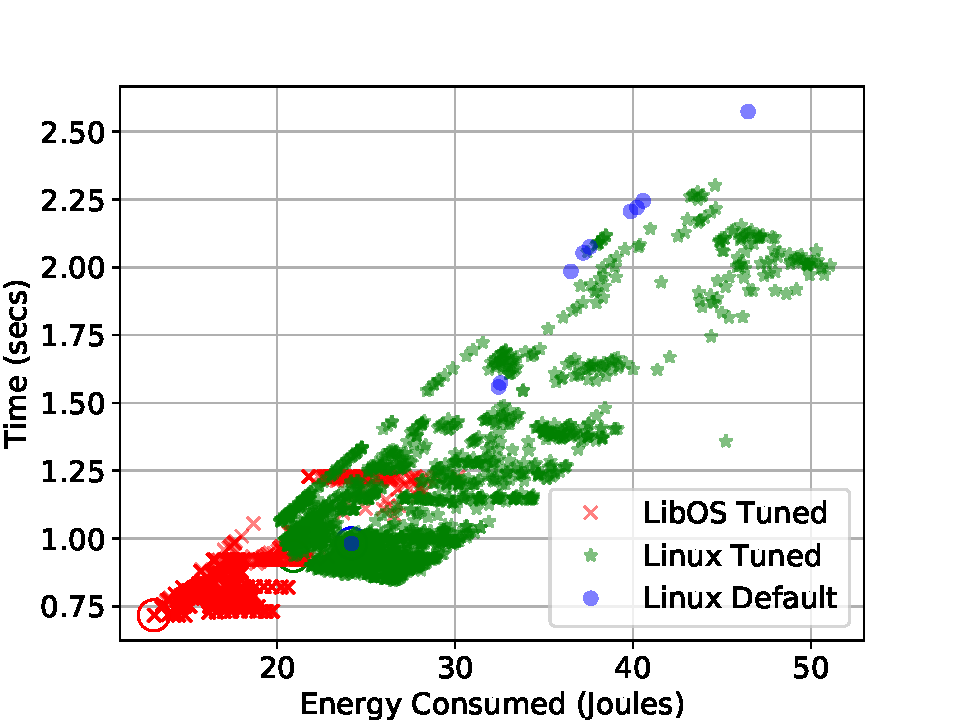
\includegraphics[width=\textwidth]{osdi_figures/netpipe_65536_overview.pdf}
        \end{subfigure}
%        \hfill
        \begin{subfigure}[b]{0.45\textwidth}  
            \centering 
            \caption[]%
            {{\small Memcached 600K QPS}} 
            \vspace*{-0.25cm}    
            \label{fig:mcdov}
            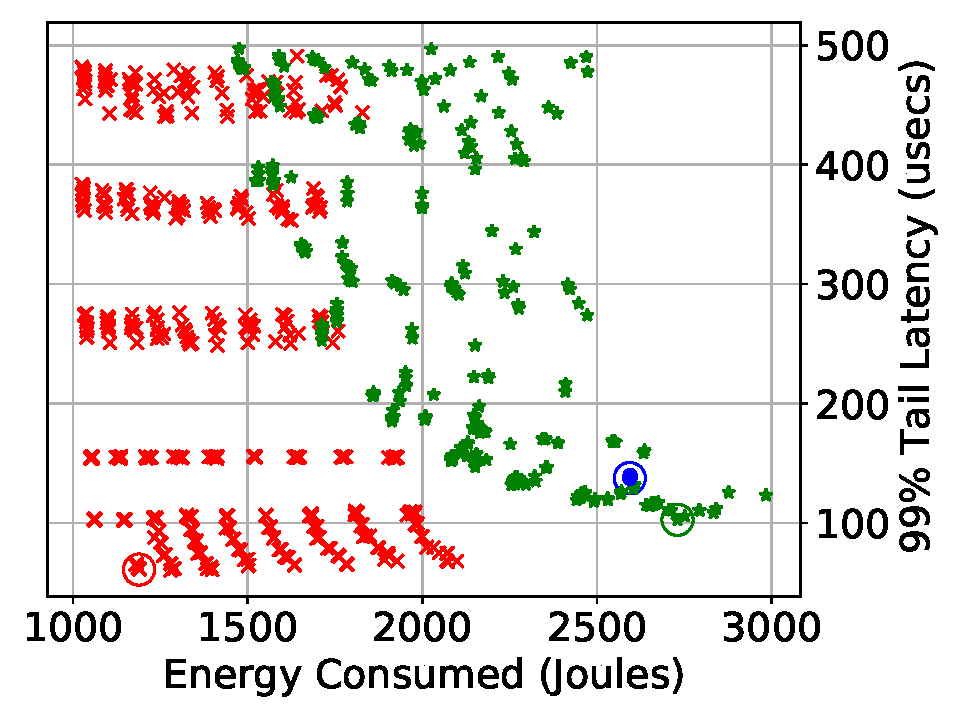
\includegraphics[width=\textwidth]{osdi_figures/mcd_600000_overview.pdf}
        \end{subfigure}
        \vskip\baselineskip
        \vspace*{-0.47cm} 
        \begin{subfigure}[b]{0.45\textwidth}   
            \centering 
            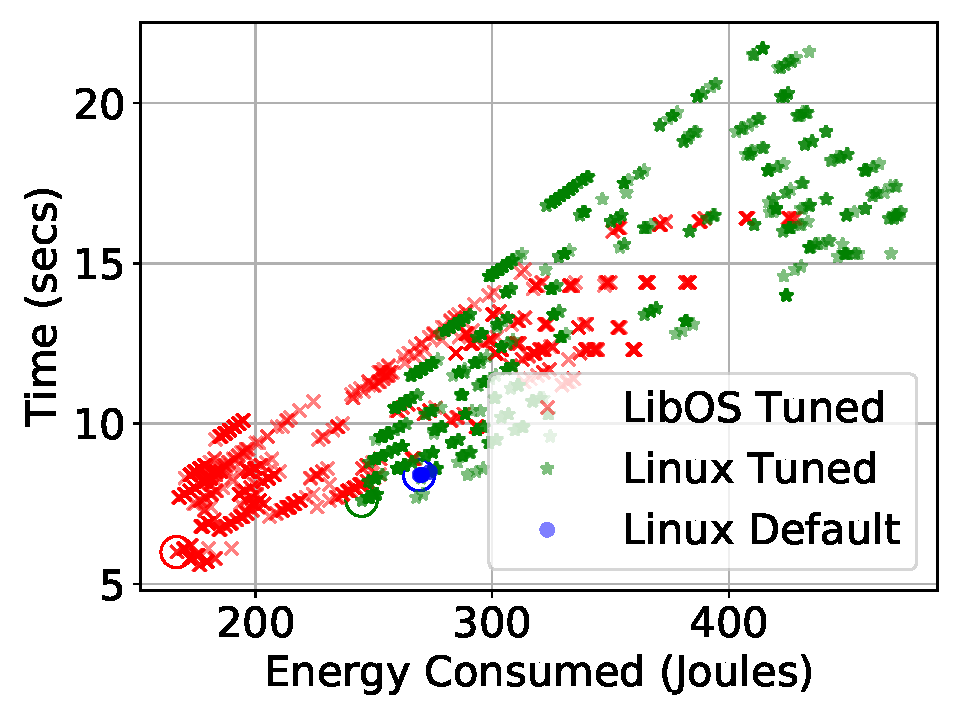
\includegraphics[width=\textwidth]{osdi_figures/nodejs_overview.pdf}
            \caption[]%
                    {{\small NodeJS 100K requests}}
                    %\hspace*{0.35cm}  
            \label{fig:nodejsov}
        \end{subfigure}
%        \hfill
        \begin{subfigure}[b]{0.45\textwidth}   
            \centering 
            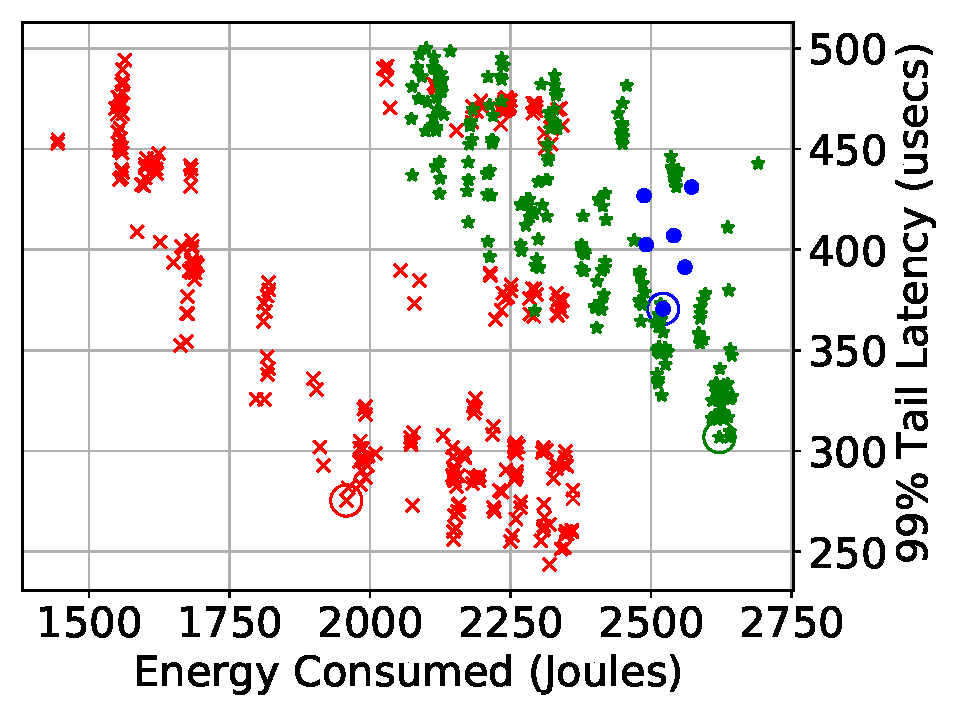
\includegraphics[width=\textwidth]{osdi_figures/mcdsilo_200000_overview.pdf}
            \caption[]%
            {{\small Memcached-silo 200K QPS}}    
            \label{fig:mcdsiloov}
        \end{subfigure}
        \caption[]
                {\small
These landscape plots portray the space of energy-performance profiles
that an OS/workload software stack can exhibit. The circle around individual points represent the min EPP values achieved in each workload.
\textit{Note that, in these plots, the origins do not start at zero
because the aim of the plots is to highlight structure within a plot
rather than to draw a comparison across plots.}
                  %Data from a run the settings associated with the 'best' EPP points are presented in~\ref{sec:data} and discussed in~\ref{sec:details}.          %Using these values we plot a timeline of the joule readings for one experimental run at the setting for Linux tuned and libOS along with data from a default Linux run of the workload.  The x-axis is the time offset from the beginning of the experiment.  For each log entry with a joule reading, we plot its value against its timestamp offset from the beginning of the run.  While the log has entries for every interrupt, we restrict sampling the joule counter to be at least 1ms apart as per the hardware manual's recommendation, as such not all log entries have an associated joule value.  To improve readability we only show a subset of the markers and use a line to connect the visible marks to the points not shown.    
        } 
        \label{fig:overview}
    \end{figure*}

